% ============================================================
% Scoped aggregation discriminability analysis
% Target: ~4 pages
% ============================================================

\section{Scoped Mechanistic Context: Aggregation Discriminability}
\label{sec:snr}

The prospective benchmark shows that the evaluated graph statistics are inadequate selection rules; it does not explain which interactions those summaries omit. As limited mechanistic context, we isolate how a linear aggregation operator changes class-conditional first and second moments in a binary fixed-degree surrogate. The calculation is exact for the stated conditional-neighbor model, but it is not an information-theoretic error bound, a model-selection rule, or a guarantee for a trained GNN.

\begin{table}[t]
\centering
\caption{Key Notation Used in This Section}
\label{tab:notation}
\small
\begin{tabular}{@{}cl@{}}
\toprule
\textbf{Symbol} & \textbf{Definition} \\
\midrule
$\rho$ & Conditional neighbor-label correlation, $\rho\in[-1,1]$ \\
$d$ & Fixed number of aggregated neighbors \\
$s$ & Feature strength, $s=\mu^\top\Sigma^{-1}\mu$ \\
$\kappa$ & Exact discriminability ratio in Proposition~\ref{prop:fixed_degree} \\
$\alpha$ & Weight on the center-node feature, $\alpha\in[0,1]$ \\
$\mathcal{D}(Z)$ & Moment-based Mahalanobis discriminability of $Z$ \\
$\Delta_Z$ & Class separation, $\mathbb{E}[Z|Y=+1] - \mathbb{E}[Z|Y=-1]$ \\
$\Sigma_Z$ & Within-class covariance, $\mathrm{Cov}(Z|Y)$ \\
\bottomrule
\end{tabular}
\end{table}

\subsection{Problem Setup}

Let the center label be $Y_v\in\{-1,+1\}$ with equal class prior and let
\begin{equation}
    X_v=Y_v\mu+\varepsilon_v,
    \qquad \varepsilon_v\sim\mathcal{N}(0,\Sigma),
\end{equation}
where $\Sigma\succ0$, $\mu\neq0$, and noises are independent across nodes. Conditional on $Y_v=y$, the $d\geq1$ neighbor labels are independent and satisfy
\begin{equation}
    \mathbb{P}(Y_i=y\mid Y_v=y)=\frac{1+\rho}{2}.
\end{equation}
Thus $\mathbb{E}[Y_i\mid Y_v=y]=\rho y$ and $\operatorname{Var}(Y_i\mid Y_v=y)=1-\rho^2$. In a balanced binary graph with a uniform conditional neighbor mechanism, $\rho$ corresponds to $2h-1$; the derivation itself is conditional and does not replace a random graph degree by its mean.

\begin{definition}[Moment-Based Discriminability]
\label{def:discriminability}
Suppose the two classes have the same nonsingular conditional covariance $\Sigma_Z$. We define the moment-based discriminability of representation $Z$ as
\begin{equation}
    \mathcal{D}(Z) := \Delta_Z^\top \Sigma_Z^{-1} \Delta_Z
\end{equation}
where $\Delta_Z = \mathbb{E}[Z|Y=+1] - \mathbb{E}[Z|Y=-1]$. This quantity uses only the first two conditional moments. It is not, in general, a distance between the full class-conditional distributions.
\end{definition}

\subsection{Exact Fixed-Degree Calculation}

We first analyze a deliberately restricted model without replacing a random degree by its expectation. Conditional on a center label $Y_v=y$, let $Y_1,\ldots,Y_d$ be independent neighbor labels satisfying $\mathbb{P}(Y_i=y\mid Y_v=y)=(1+\rho)/2$. Let $X_i=Y_i\mu+\varepsilon_i$, where the $\varepsilon_i\sim\mathcal{N}(0,\Sigma)$ are independent of all labels, and define $A_v=d^{-1}\sum_{i=1}^d X_i$.

\begin{proposition}[Exact Fixed-Degree Discriminability]
\label{prop:fixed_degree}
For $s=\mu^\top\Sigma^{-1}\mu>0$, the conditional moments and discriminability ratio are
\begin{align}
    \mathbb{E}[A_v\mid Y_v=y] &= \rho y\mu,\\
    \operatorname{Cov}(A_v\mid Y_v=y)
        &= \frac{1}{d}\left(\Sigma+(1-\rho^2)\mu\mu^\top\right),\\
    \kappa(d,\rho,s)
        :=\frac{\mathcal{D}(A)}{\mathcal{D}(X)}
        &=\frac{\rho^2d}{1+(1-\rho^2)s}.
\end{align}
\end{proposition}

\begin{proof}
We derive this result in three steps.

Since $\mathbb{E}[Y_i\mid Y_v=y]=\rho y$ and
$\operatorname{Var}(Y_i\mid Y_v=y)=1-\rho^2$, independence gives the first two identities. Moreover, $\Delta_X=2\mu$, $\mathcal{D}(X)=4s$, and $\Delta_A=2\rho\mu$. Applying the Sherman--Morrison identity,
\begin{equation}
 \mu^\top\left(\Sigma+(1-\rho^2)\mu\mu^\top\right)^{-1}\mu
 =\frac{s}{1+(1-\rho^2)s}.
\end{equation}
Substitution yields the stated ratio.
\end{proof}

\subsection{Center-Feature and Neighbor Mixing}

Neighbor-only averaging does not represent a self-looped GCN layer. To isolate the effect of retaining the center feature, consider the analyzable linear surrogate
\begin{equation}
    Z_{\alpha,v}=\alpha X_v+(1-\alpha)A_v,
    \qquad \alpha\in[0,1].
    \label{eq:self_neighbor_operator}
\end{equation}
The scalar $\alpha$ is a prescribed mixing weight; it is not identified with a learned GCN coefficient.

\begin{proposition}[Exact Self--Neighbor Mixing Discriminability]
\label{prop:self_neighbor_mixing}
Under the fixed-degree model above, assume that the center-feature noise is conditionally independent of all neighbor labels and features. Define
\begin{align}
    m_\alpha &= \alpha+(1-\alpha)\rho,\\
    c_\alpha &= \alpha^2+\frac{(1-\alpha)^2}{d},\\
    q_\alpha &= \frac{(1-\alpha)^2(1-\rho^2)}{d}.
\end{align}
Then
\begin{align}
    \mathbb{E}[Z_{\alpha,v}\mid Y_v=y]
        &=m_\alpha y\mu,\\
    \operatorname{Cov}(Z_{\alpha,v}\mid Y_v=y)
        &=c_\alpha\Sigma+q_\alpha\mu\mu^\top,
\end{align}
and the exact moment-based discriminability ratio is
\begin{align}
    \kappa_\alpha(d,\rho,s)
    &:=\frac{\mathcal{D}(Z_\alpha)}{\mathcal{D}(X)} \notag\\
    &=\frac{[\alpha+(1-\alpha)\rho]^2}
    {\alpha^2+(1-\alpha)^2/d
    +[(1-\alpha)^2/d](1-\rho^2)s}.
    \label{eq:kappa_alpha}
\end{align}
\end{proposition}

\begin{proof}
Conditional independence makes the center and neighbor covariance contributions additive, which gives the stated mean and covariance. For
$B=c_\alpha\Sigma+q_\alpha\mu\mu^\top$, the Sherman--Morrison identity gives
\begin{equation}
    \mu^\top B^{-1}\mu=\frac{s}{c_\alpha+q_\alpha s}.
\end{equation}
Since the class-mean difference is $2m_\alpha\mu$, we have
$\mathcal{D}(Z_\alpha)=4m_\alpha^2s/(c_\alpha+q_\alpha s)$. Dividing by $\mathcal{D}(X)=4s$ proves~\eqref{eq:kappa_alpha}.
\end{proof}

The boundary cases provide checks on the formula. Setting $\alpha=0$ recovers Proposition~\ref{prop:fixed_degree}; setting $\alpha=1$ gives $\kappa_\alpha=1$; and $|\rho|=1$ removes label-mixture covariance. A negative $\rho$ can also cancel the center and neighbor class means when $m_\alpha=0$, showing why self-loops do not uniformly prevent damage.

\begin{corollary}[Discriminability Transition]
\label{cor:threshold}
In the fixed-degree model, aggregation improves Mahalanobis discriminability exactly when
\begin{align}
    \kappa>1
    &\iff \rho^2 > \frac{1+s}{d+s}.
\end{align}
Thus the transition depends on feature strength as well as degree and edge correlation. The simpler condition $\rho^2d>1$ is recovered only as $s\to0$.
\end{corollary}

\begin{table}[t]
\centering
\caption{Exact Discriminability-Loss Region Depends on Feature Strength}
\label{tab:threshold}
\begin{tabular}{@{}ccc@{}}
\toprule
$(d,s)$ & Boundary $|2h-1|$ & Loss Region ($h$) \\
\midrule
$(10,0^+)$ & 0.316 & (0.34, 0.66) \\
$(10,1)$ & 0.426 & (0.29, 0.71) \\
$(10,4)$ & 0.598 & (0.20, 0.80) \\
$(20,1)$ & 0.309 & (0.35, 0.65) \\
\bottomrule
\end{tabular}
\end{table}

\textbf{Interpretation} (Table~\ref{tab:threshold}): The first row is the limit as $s\to0^+$ because the ratio itself is undefined when both class representations have zero discriminability. Stronger self-feature separation increases the label-mixture penalty and widens the region in which neighbor-only aggregation loses discriminability. This is a property of the stated moment criterion, not a universal guarantee for a trained GNN.

\subsection{Approximation Regime}

The exact ratio satisfies
\begin{equation}
 \frac{\rho^2d}{1+\eta}\leq\kappa\leq\rho^2d,
 \qquad \eta=(1-\rho^2)s.
\end{equation}
Consequently, the exact ratio falls below the approximation by the fraction
$(\rho^2d-\kappa)/(\rho^2d)=\eta/(1+\eta)$, while the approximation overstates the exact value by $(\rho^2d-\kappa)/\kappa=\eta$. This makes the required feature-noise-dominance regime explicit and does not invoke an asymptotic $o(1)$ term.

\subsection{Direct Moment Validation}

We test the implemented formulas on a frozen grid rather than infer validity from downstream GNN accuracy. The grid contains 400 configurations over degree, edge-label correlation, feature strength, and center-feature weight, with five fixed seeds and 5,000 samples per class. All 2,000 configuration--seed records complete successfully and retain the empirical moments, exact prediction, environment, and source commit. Across the 1,920 records with a nonzero exact ratio, the median absolute relative error between the empirical estimate and $\kappa_\alpha$ is 0.94\% (descriptive 95\% percentile-bootstrap interval 0.86--1.05\%). In the neighbor-only slice, the median absolute error of the simplified $\rho^2d$ approximation is 0.293 (0.242--0.365), and its overstatement increases with feature strength.

\begin{figure}[t]
\centering
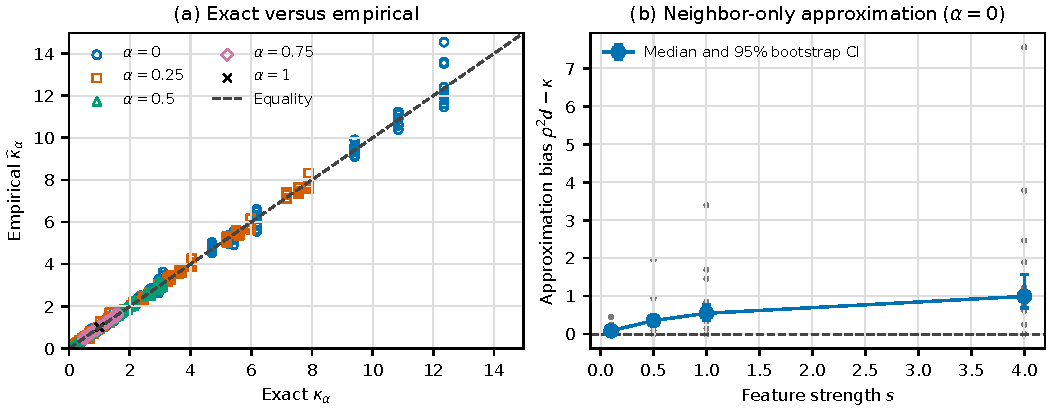
\includegraphics[width=\linewidth]{results/discriminability/route_a_grid_v1/summary/validation_figure}
\caption{Frozen moment validation. Left: empirical and exact $\kappa_\alpha$. Right: signed error of the neighbor-only $\rho^2d$ approximation, with descriptive bootstrap intervals of the median.}
\label{fig:direct_discriminability_validation}
\end{figure}

This experiment validates the implemented first- and second-moment calculation within the prescribed surrogate grid. It does not validate a Bayes-error formula, a trained-GNN performance law, or a graph-vs-MLP selector.

\subsection{Broadcasting Context, Not a GNN Threshold}

The product ``branching factor $\times$ squared label correlation'' also appears in classical tree broadcasting and reconstruction. For a regular tree with forward branching factor $b$, the Kesten--Stigum quantity is $b\rho^2$~\cite{kesten1966additional,mossel2015reconstruction}. Here $b=q-1$ for a $q$-regular undirected tree, whereas a Poisson Galton--Watson limit with mean offspring $k$ uses $b=k$. This resemblance supplies historical context for the weak-feature limit of our one-hop ratio; it is not a new threshold result. In particular, $d$ in Proposition~\ref{prop:fixed_degree} is a fixed one-hop neighbor count and must not be interchanged with either forward degree without an explicit coupling. Ordinary finite-depth GNNs also reuse neighborhoods and may include self-loops, normalization, nonlinearities, attention, and learned transformations. We therefore derive no Kesten--Stigum condition for GNN depth or architecture. Recent finite-depth CSBM analysis likewise finds Gaussian-mixture embeddings and depth behavior more complex than a single-Gaussian account~\cite{pmlr-v269-dalle25a}.

\subsection{Extensions Not Claimed Here}

A multi-class graph is described by a class-transition matrix rather than one scalar edge correlation. Collapsing that matrix to homophily can hide which class pairs are mixed and how their feature means are arranged. We therefore do not present a scalar multi-class threshold. Likewise, a practical GCN introduces variable degree, self-loop normalization, learned transformations, nonlinearities, and neighborhood reuse across layers. Proposition~\ref{prop:self_neighbor_mixing} isolates a prescribed self-feature weight but does not remove these remaining differences.

\subsection{Scope and Random-Degree Extension}

The class-conditional distribution of $A_v$ is generally a Gaussian mixture because the neighbor labels are random. Therefore the Gaussian Bayes-error formula stated for $X_v$ must not be applied to $A_v$ solely from its first two moments. Proposition~\ref{prop:fixed_degree} concerns Mahalanobis discriminability only.

For sparse CSBM, the degree is random. Conditional on $D_v=m>0$, Proposition~\ref{prop:fixed_degree} applies with $d=m$. An unconditional calculation must specify the treatment of isolated nodes and average over the degree-conditioned mixture; replacing $D_v$ by its mean is not exact. We leave that random-degree extension separate rather than attach unsupported finite-$n$ error rates to the fixed-degree result.
